\documentclass{article}
\usepackage{amsmath}
\usepackage{amsthm}
\usepackage{multicol}
\usepackage{natbib}
\setcitestyle{square}

\usepackage{minted}
\usemintedstyle{manni}

\usepackage[charter]{mathdesign}
\DeclareSymbolFont{usualmathcal}{OMS}{cmsy}{m}{n}
\DeclareSymbolFontAlphabet{\mathcal}{usualmathcal}

\usepackage{microtype}

\usepackage[left=.5in,right=.5in,top=.5in,bottom=1in]{geometry}

\newcommand{\ie}{\emph{i.e.}}
\newcommand{\eg}{\emph{e.g.}}
\newcommand{\etc}{\emph{etc.}}

\addtolength{\parskip}{\baselineskip}

\usepackage{graphicx}
\usepackage{subcaption}

\DeclareCaptionFormat{custom}
{%
    \textbf{#1#2}\textit{#3}
}
\captionsetup{format=custom}

\title{A Simple Parametric Model of Plain-Knit Yarns}
\author{Keenan Crane}

\begin{document}

\maketitle

\begin{figure}[h!]
   \centering
   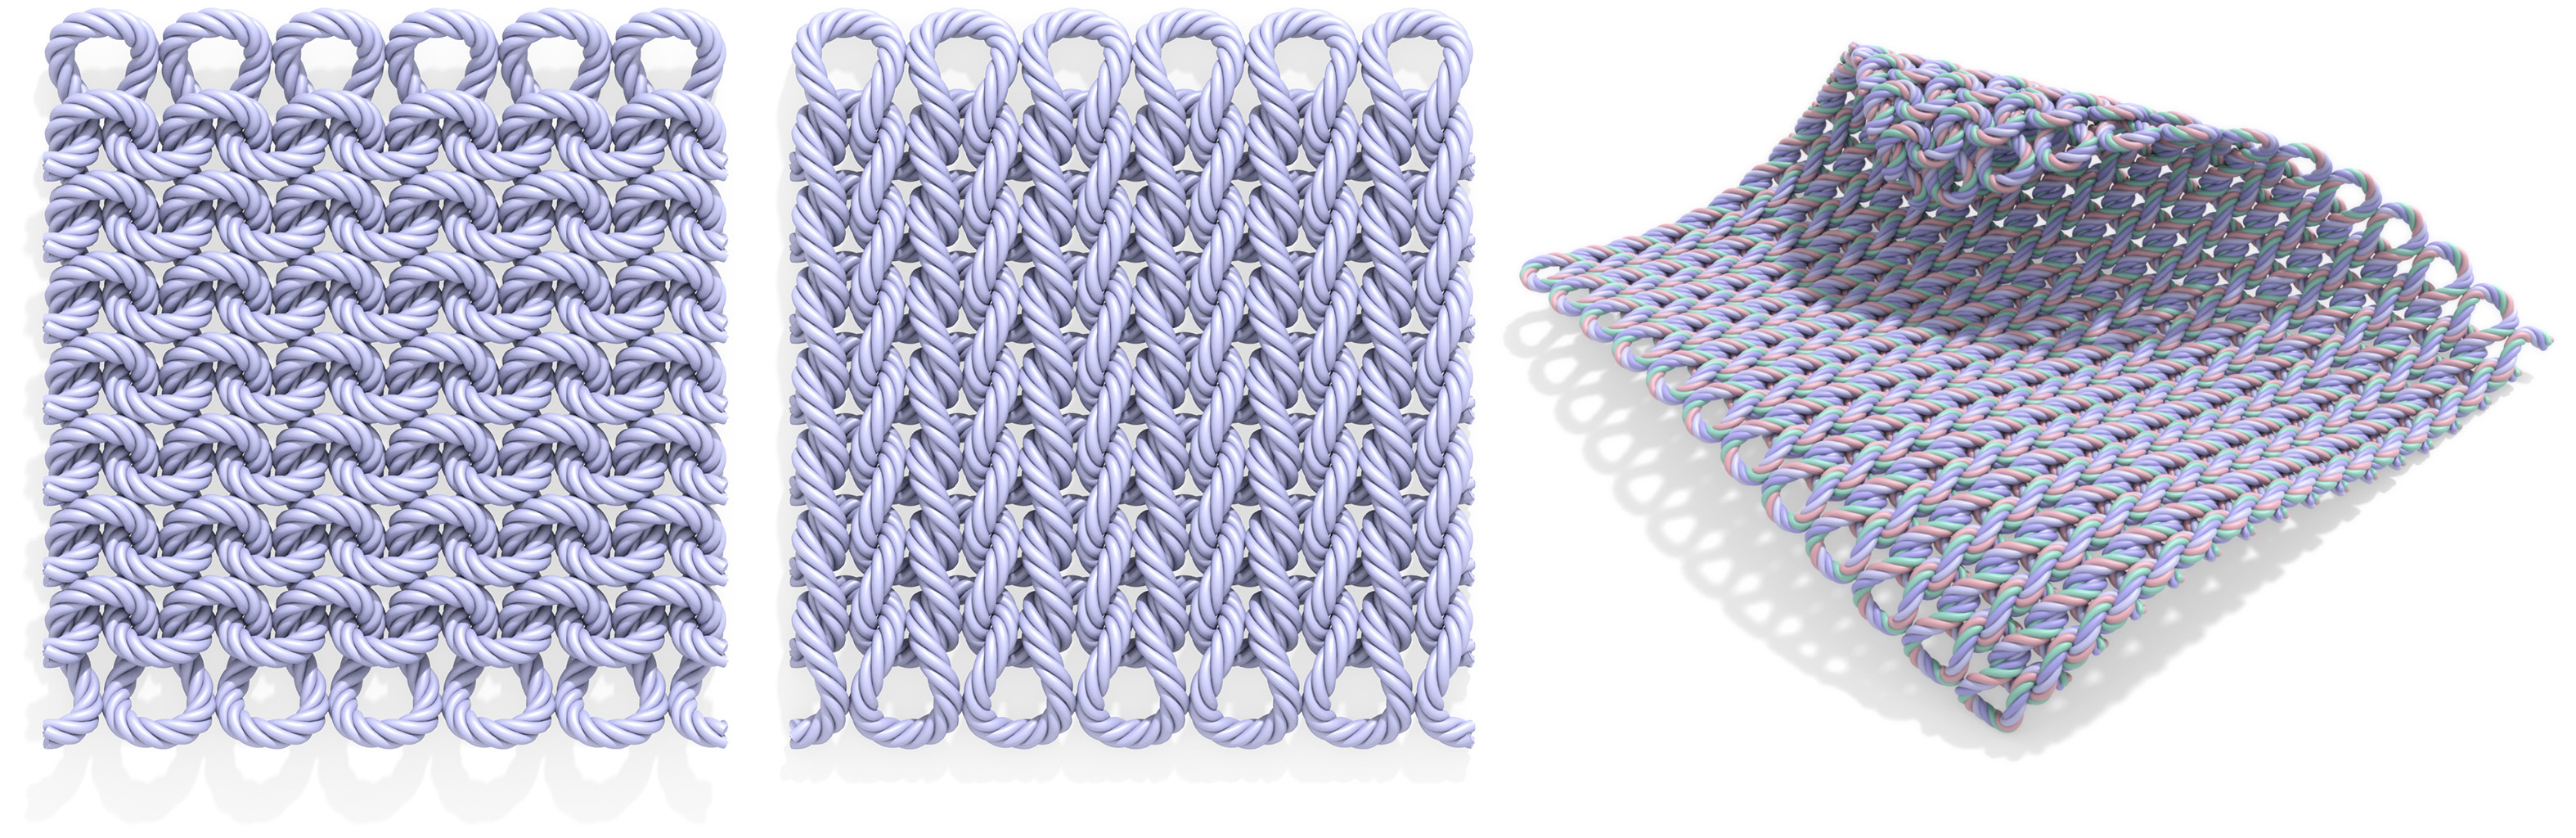
\includegraphics[width=.8\textwidth]{images/teaser.jpg}
   \caption{Plain knit yarns viewed from the back \emph{(left)}, front \emph{(center)}, and mapped onto a developable surface \emph{(right)}.\label{fig:teaser}}
\end{figure}

\textbf{Abstract:} \emph{This short note gives closed-form expressions for smooth curves resembling a plain-knit stitch, suitable for appearance modeling and previsualization.  A unique feature of this model is that it also describes the twisted yarn fibers running along this stitch, making it suitable for modeling marled yarn. Adjustable parameters control the knit spacing, loop roundness, yarn thickness, and rate of fiber twisting.  Tileable displacement maps and code for generating curves are also provided.}

\section{Overview}

A \emph{plain stitch}, also known as a \emph{stockinette stitch}, \emph{jersey stitch}, \emph{flat stitch}, or \emph{felt stitch}, is a basic knitting pattern formed by rows of identical yarn loops.  Though a beautiful array of decorative knit stitches appear in the design of textiles, the plain stitch is the baseline pattern used for common garments, upholstery, \etc{}\  Hence, visual simulation of everyday objects can benefit from a cheap, simple, and controllable model of the kind presented here.  Parameterization of twisted fibers makes our model especially suitable for \emph{marled} yarns, where several fibers or \emph{rovings} of different color are twisted together to form a single yarn.

The geometry of the plain stitch pattern arises from an interplay between elastic forces (bending and twisting of a rod) and collision forces (frictional contact between neighboring yarns), and has in the past been modeled via numerical optimization~\citep{yuksel2012stitch}, physical simulation~\citep{kaldor2010efficient}, and via a helicoid model~\citep{wadekar2020geometric}.  Parametric models have long been used in the textile industry to understand and predict physical properties of knitted garments (dimensions, weight, material usage, \etc{}).  For instance, \citet{Chamberlain:1926:HYF} gives a 2D description that is useful for reasoning about material properties, but not sufficient for capturing 3D appearance.  To our knowledge, the first parameterization of a three-dimensional plain knit stitch was given by \citet[Part IV]{Peirce:1947:GPA}, as a 2D piecewise function with straight and circular parts, composed with a mapping to a 3D cylinder.  The lack of curvature continuity, and the piecewise nature of this function, makes it difficult to develop a parameterization of the secondary twisted fibers.  Moreover, Peirce's curve does not provide many parameters to adjust the shape or appearance of the knit pattern (only the yarn diameter and wale/course spacing).  On the other hand, geometrically simple components make the curve and its parameters easy to analyze, whereas quantities like arc length and maximal thickness must be determined numerically for our model (Section \ref{sec:ArcLengthAndThickness}).  \citet{Leaf:1955:GPK} and \citet{Munden:1959:GDP} refine Peirce's model and connect it to empirical data; Munden in particular observes that yarn shape is largely geometric and variational in nature, \ie, arising from energy minimization that does not depend strongly on yarn properties or stitch length.  Twisted fibers can be seen in many papers from the computer graphics literature (\eg{}, \citet{kaldor2010efficient}), but no explicit equations are given.  In general, we were unable to find any parameterized version of the twisted fiber curves in the literature, though given the cultural importance of knitting it is very likely that such a parameterization has been written down somewhere. 

In this note, the geometry of each row (corresponding to the course direction) is given as a parameterization of the centerline, \ie, the curve passing through the center of the yarn; the geometry of the yarn itself can be approximated by a tubular neighborhood of some radius \(R > 0\) around this centerline.  Multiple copies of this curve, offset along the wale direction, can be used to model a piece of knitted material.  Secondary curves describe the centerlines of individual fibers; here, a simple correction to the Frenet frame yields a good approximation to the twist-free (Bishop) frame---providing a near-uniform rate of twist around the yarn centerline (Section~\ref{sec:YarnFibers}).  Though our parameterization has no direct physical origin (\eg, it does not minimize a potential energy), it nonetheless captures the appearance of real knit yarn reasonably well at intermediate scales (see \citep{zhao2016fitting} for models of yarn microstructure, and \citep{xu2001photorealistic,jakob2010radiative} for a discussion of photorealistic rendering).  Moreover, a closed-form expression is efficient to evaluate, has well-defined derivatives of all orders, has easily-adjustable parameters, and lends itself well to constructing secondary curves describing twisted yarn fibers (which are difficult or expensive to capture via optimization and simulation).  This pattern can then be mapped onto a surface to obtain an appearance similar to a knit garment---Figure \ref{fig:teaser}, \emph{right} shows an example achieved by composing the yarn curve with a parameterized developable surface, using the \(z\)-coordinate of the curve to determine an offset in the normal direction.  If more physical results are desired, these initial curves can be further optimized or simulated to better match the behavior of physical yarn~\citep{kaldor2010efficient,yuksel2012stitch}.  Appendex \ref{app:DisplacementMaps} provides displacement maps that can be used for finer patterns (or on more complex geometry).

\section{Yarn}
\label{sec:Yarn}

To develop a parameterized yarn, we start with a simple sinusoid 
\[
   t \mapsto (t,h\cos(t),0),
\]
parameterized over values \(t \in \mathbb{R}\), where \(h > 0\) controls the height of the loops:

\begin{center}
   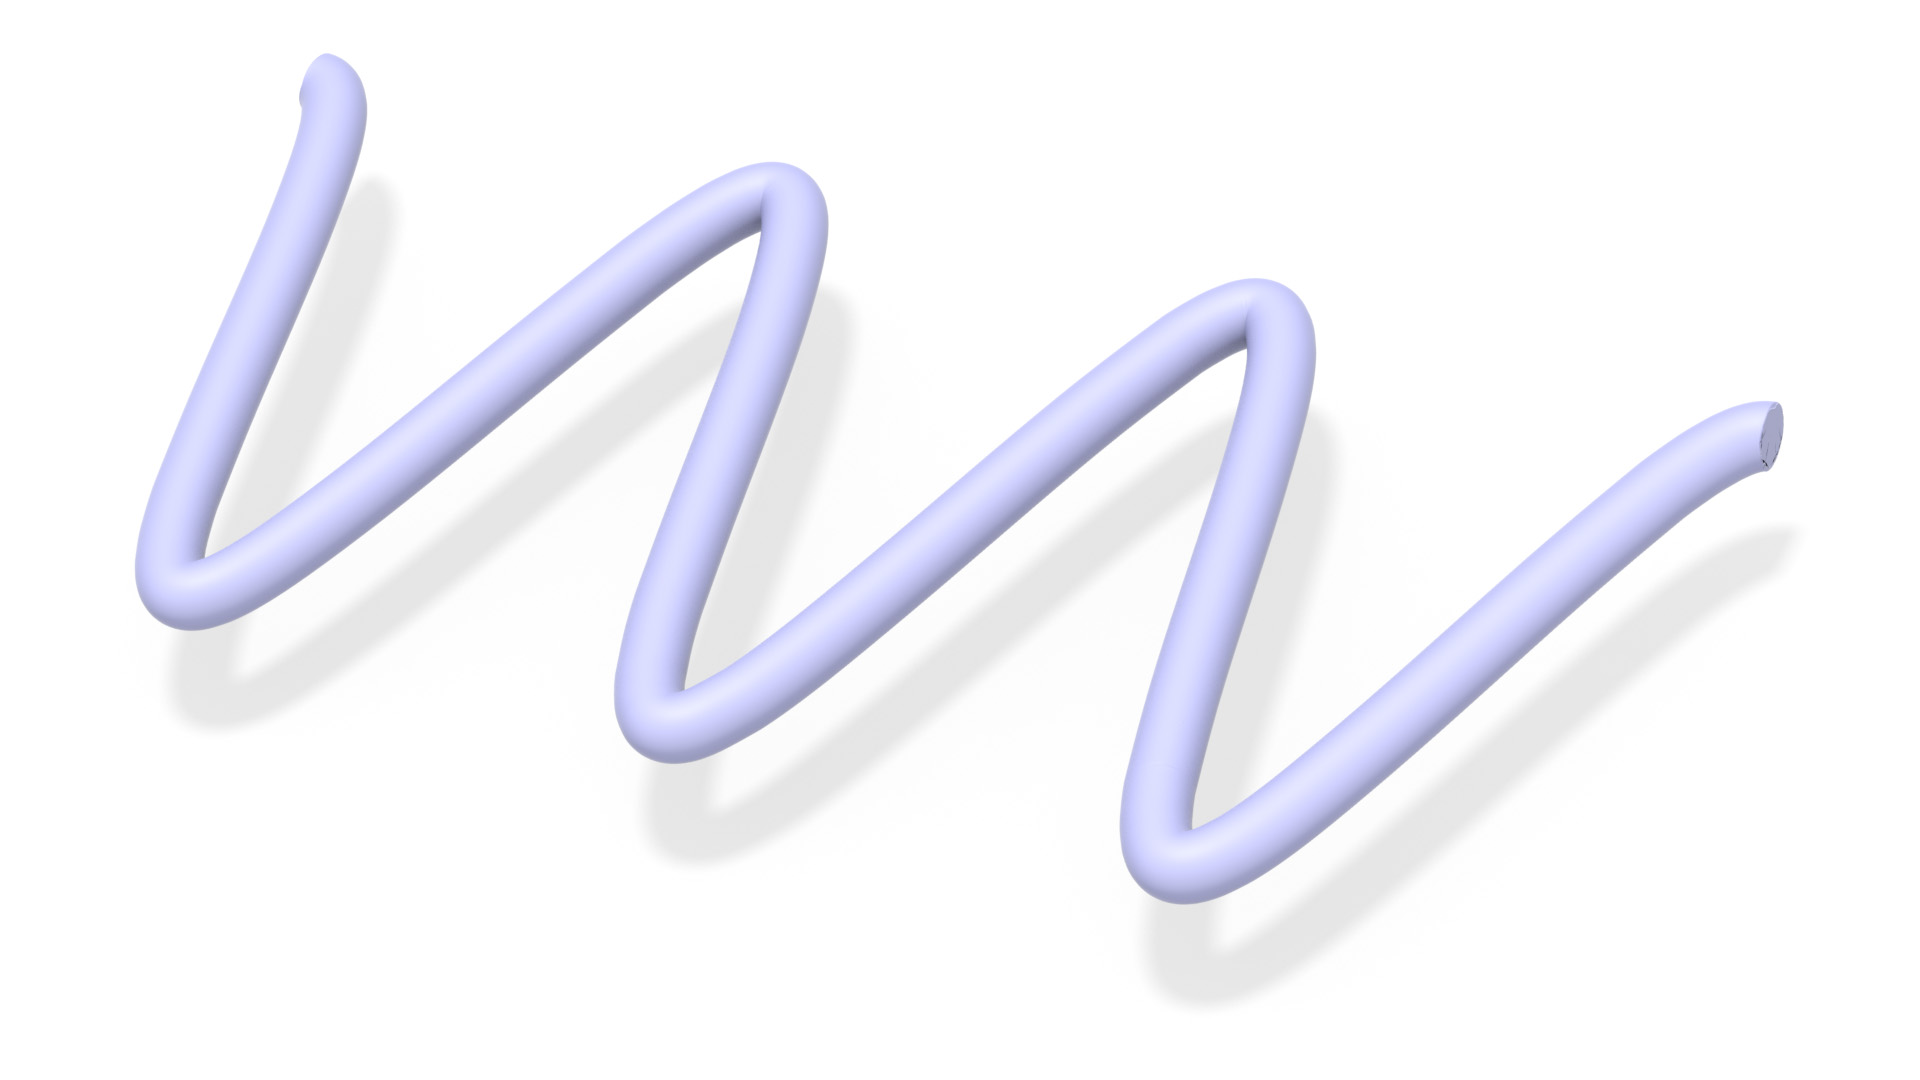
\includegraphics[width=2.5in]{images/centerline-cosine.jpg}
\end{center}

To get rounder loops, we can modify the \(x\)-coordinate so that it ``overshoots'' at the end of each loop, and ``backtracks'' slightly before making the next loop.  For instance, we can add some multiple \(a\) of \(\sin(2t)\) to get a curve
\[
   t \mapsto (t + a\sin(2t),h\cos(t),0).
\]

\begin{center}
   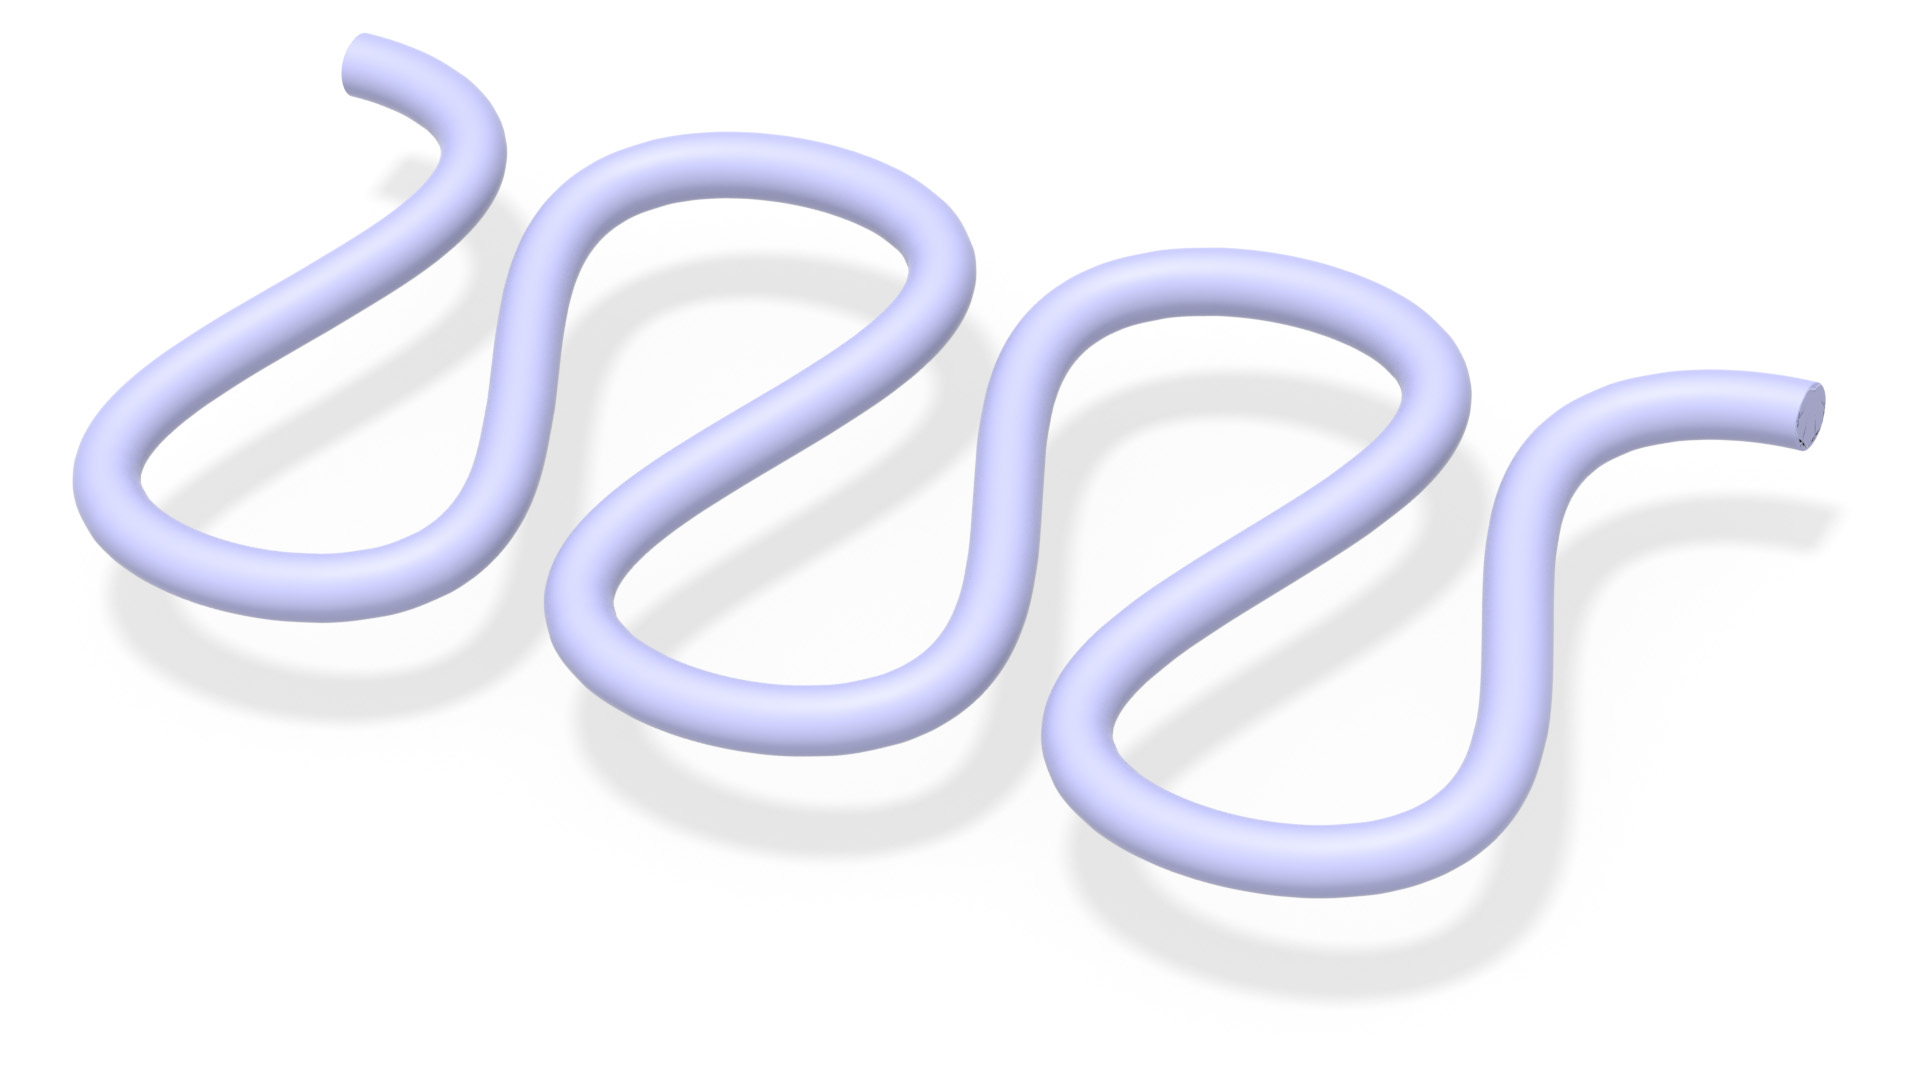
\includegraphics[width=2.5in]{images/centerline-flat.jpg}
\end{center}

Finally, in order for each row to loop around the next, the curve must bend out of plane.  We can model this bending by a sinusoid \(\cos(2t)\) in the \(z\)-direction of twice the frequency as in the wale (\(y\)) direction, with some magnitude \(d > 0\):

\begin{center}
   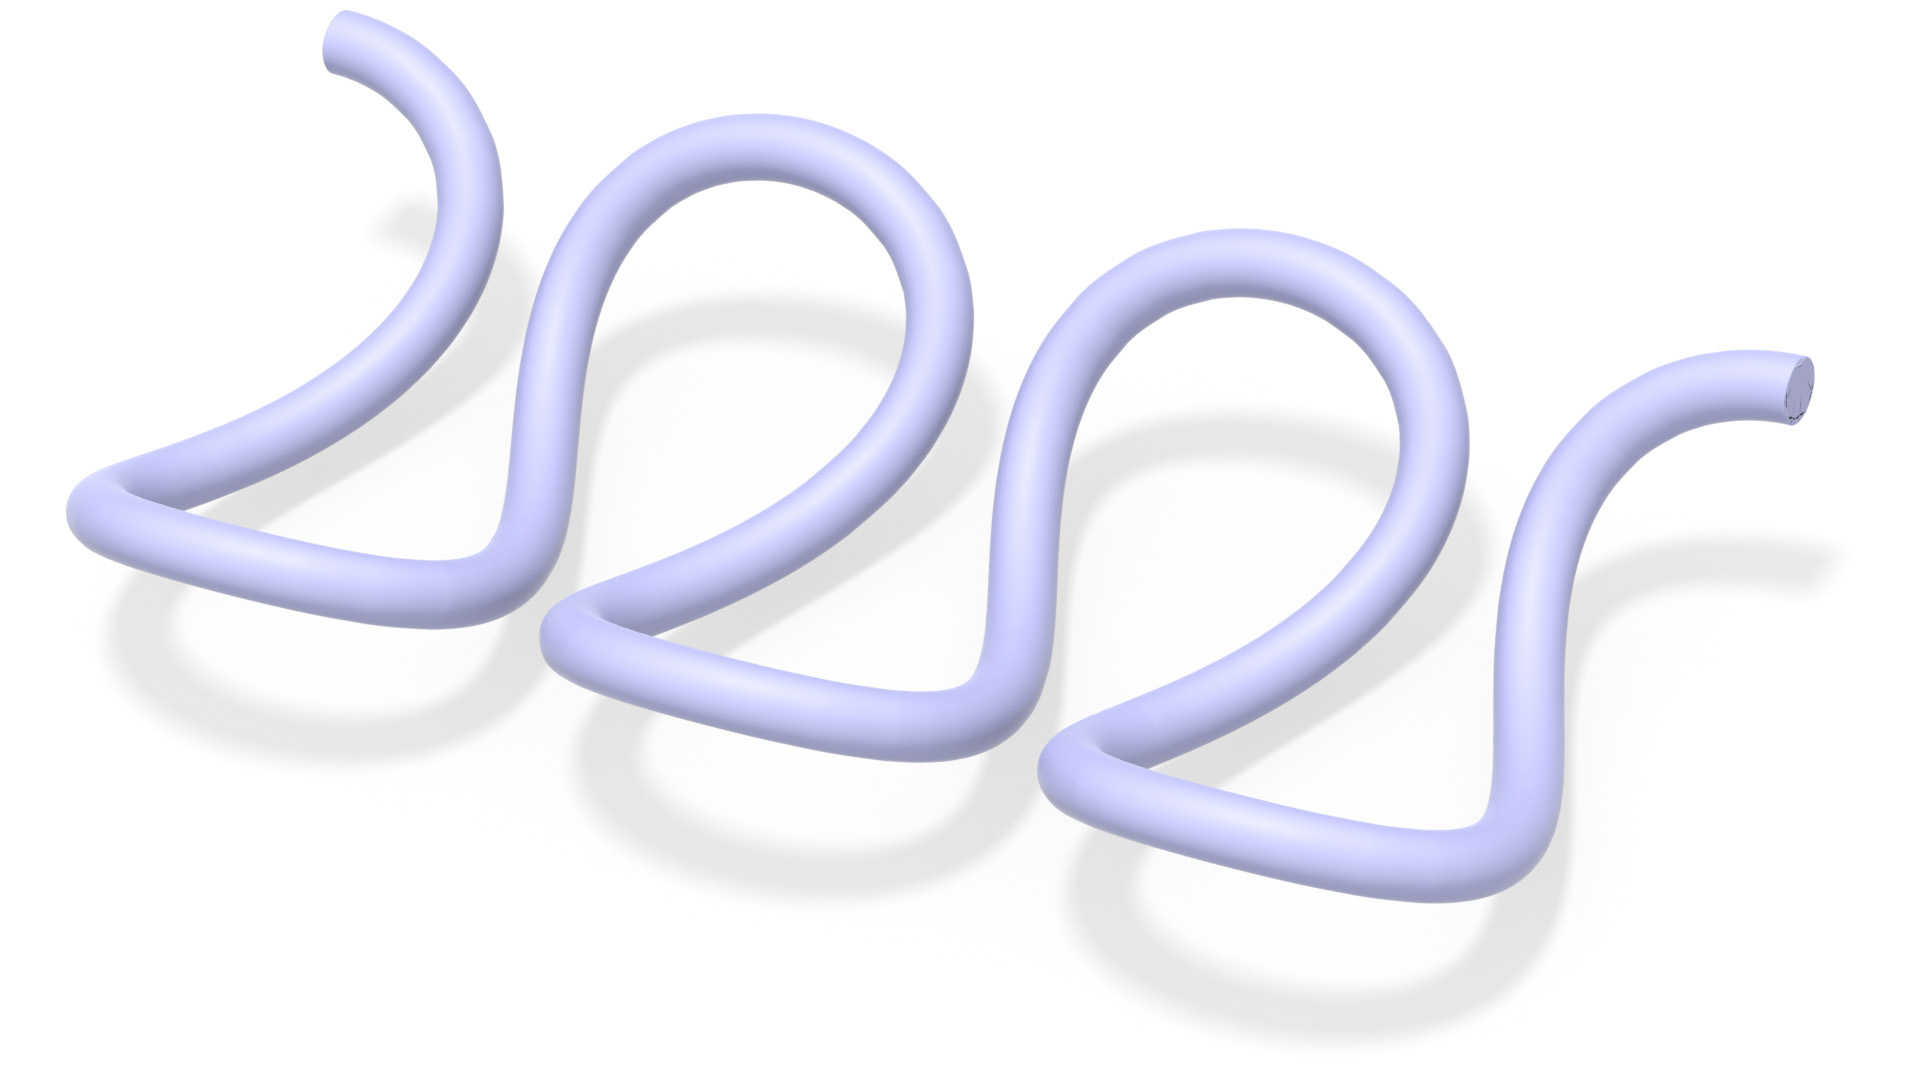
\includegraphics[width=2.5in]{images/centerline-bent.jpg}
\end{center}

The final yarn centerline is then parameterized by a curve \(\gamma: \mathbb{R} \to \mathbb{R}^3\), given by
\begin{equation}
   \boxed{\gamma(t) := \left( t + a\sin(2t), h\cos(t), d\cos(2t) \right).}
\end{equation}
The parameter \(a\) controls the roundness of the loops, the parameter \(h > 0\) controls the height of the yarn in the wale direction, and the parameter \(d > 0\) controls the depth of oscillations in and out of the plane.  Figure~\ref{fig:yarn-example} shows an example.

\begin{figure}[h!]
   \centering
   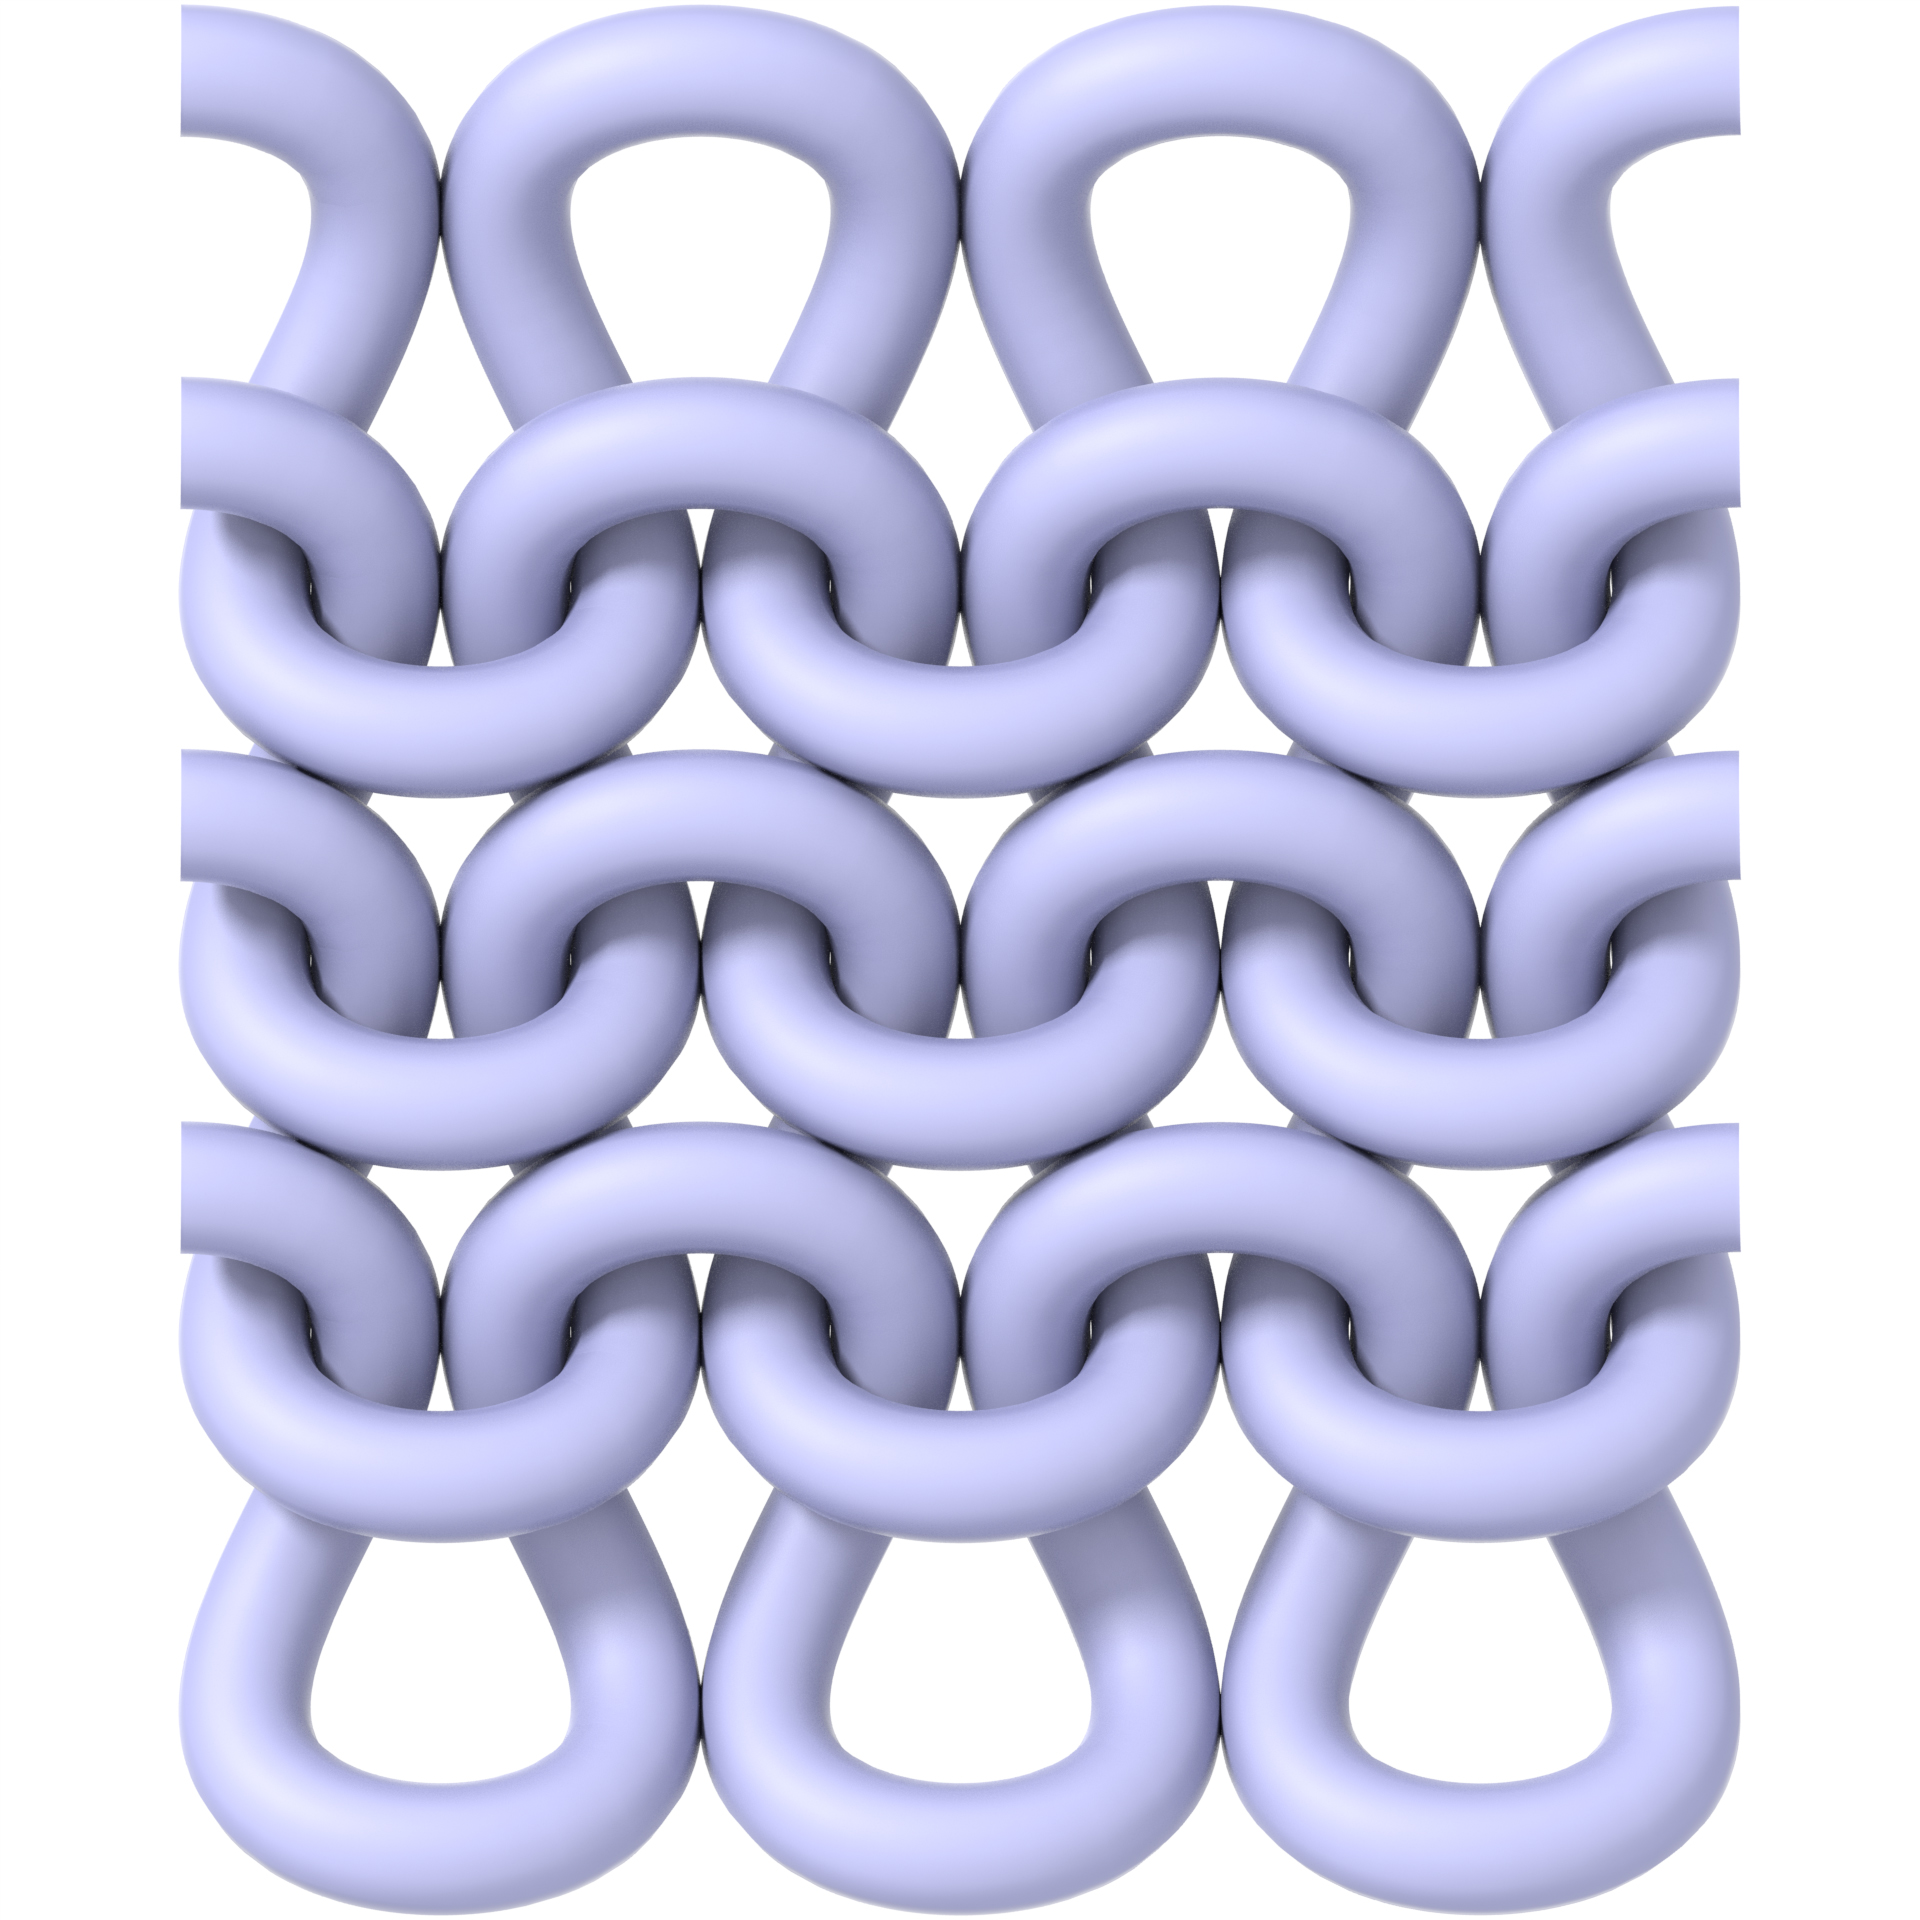
\includegraphics[width=2.5in]{images/yarn-example.jpg}
   \caption{Several copies of the yarn curve \(\gamma(t)\) for \(a=3/2\), \(h = 4\) and \(d=1\).  For a tube radius \(R = 4/5\), offsetting rows by \(h+1/2\) in the wale direction (\ie, \(y\)-direction) generally yields a snug fit between curves.\label{fig:yarn-example}}
\end{figure}

\section{Yarn Fibers}
\label{sec:YarnFibers}

\subsection{Frenet Frame}
\label{sec:FrenetFrame}

To describe a curve winding around the yarn, we first construct the Frenet frame for \(\gamma(t)\), given by three orthonormal vectors
\[
   e_1(t) := \frac{\frac{d}{dt} \gamma(t)}{\left|\frac{d}{dt} \gamma(t)\right|}, \qquad e_2(t) = \frac{\frac{d}{dt} e_1(t)}{\left|\frac{d}{dt} e_1(t)\right|}, \qquad e_3(t) := e_1(t) \times e_2(t).
\]
these directions describe the tangent, normal, and binormal of \(\gamma(t)\), respectively.  (note that to define \(e_1\) we must normal \(d\gamma/dt\), since \(\gamma\) is not an arc-length parameterized curve.)  The unnormalized directions \(\tilde{e}_1,\tilde{e}_2\) are given by
\[
   \begin{array}{rcl}
      \tilde{e}_1(t) &=& \left( 1 + 2 a \cos(2t), -h \sin(t), -2d\sin(2t) \right), \\
      \tilde{e}_2(t) &=& -\frac{v(t)}{2 u(t)^{3/2}} \left((1 + 2 a \cos(2 t)), -h \sin(t), -2 d \sin(2 t)\right) - \frac{1}{u(t)^{1/2}} \left(4 a \sin(2 t), h \cos(t), 4 d \cos(2 t)\right),
   \end{array}
\]
where
\[
   \begin{array}{rcl}
      u(t) &:=& (1 + 2 a \cos(2t))^2 + h^2 \sin(t)^2 + 4 d^2 \sin(2t)^2 \\
      v(t) &:=& 2 h^2 \cos(t) \sin(t) + 16 d^2 \cos(2 t) \sin(2 t) - 8 a (1 + 2 a \cos(2 t)) \sin(2 t). \\
   \end{array}
\]
applying the normalizations \(e_1 = \tilde{e}_1/|\tilde{e}_1|\) and \(e_2(t) = \tilde{e}_2/|\tilde{e}_2|\) and taking the cross product \(e_3 = e_1 \times e_2\) then gives an orthonormal frame.

\subsection{Fiber Curves}
\label{sec:FiberCurves}

Using the Frenet frame, a curve twisting around \(\gamma(t)\) can be expressed as
\[
   t \mapsto \gamma(t) + r( \cos(\theta(t)) e_2(t) + \sin(\theta(t)) e_3(t) ),
\]
where \(r\) is the yarn thickness, and \(\theta(t)\) is some function that gives the angular location of the fiber relative to the local frame of \(\gamma(t)\) at time \(t\).  Suppose we let \(\theta(t) = \omega t\), where \(\omega > 0\) controls the rate of twisting.  Then we almost get the behavior we want, except that there are a different number of twists on either side of the loop:

\begin{center}
   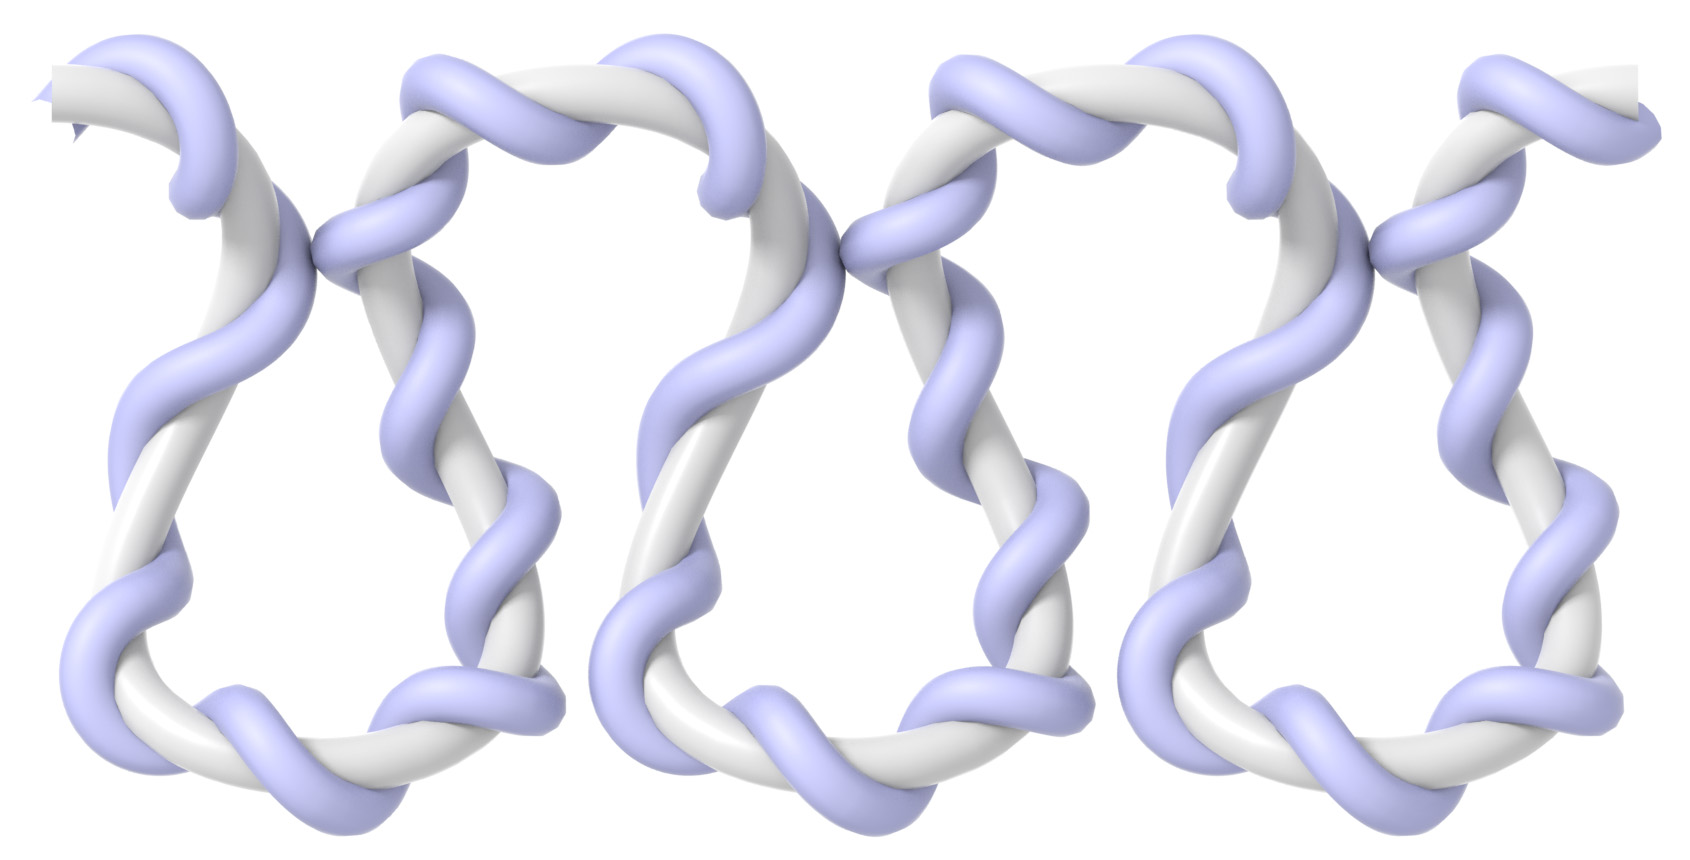
\includegraphics[width=2.5in]{images/fiber-uneven.jpg}
\end{center}

Even though the angular velocity \(\omega\) is constant, the apparent non-uniformity arises from the fact that the Frenet frame does not turn at a constant speed along the curve (Figure \ref{fig:frenet-frame}, \emph{left}).  One way to rectify this situation would be to use the \emph{Bishop frame} (\ie, frame of least twist) rather than the Frenet frame to define the yarn fibers.  However, the Bishop frame requires global integration along the curve (and these integrals generally are not available in closed form), whereas the Frenet frame can be evaluated locally at each point.  Hence, we instead approximately correct for the twisting of the Frenet frame by simply adjusting the angle of rotation by a term \(-2\cos(t)\), yielding an overall angle function \(\theta(t) = \omega t - 2\cos(t)\) (Figure \ref{fig:frenet-frame}, \emph{right}).

\begin{figure}[h!]
   \centering
   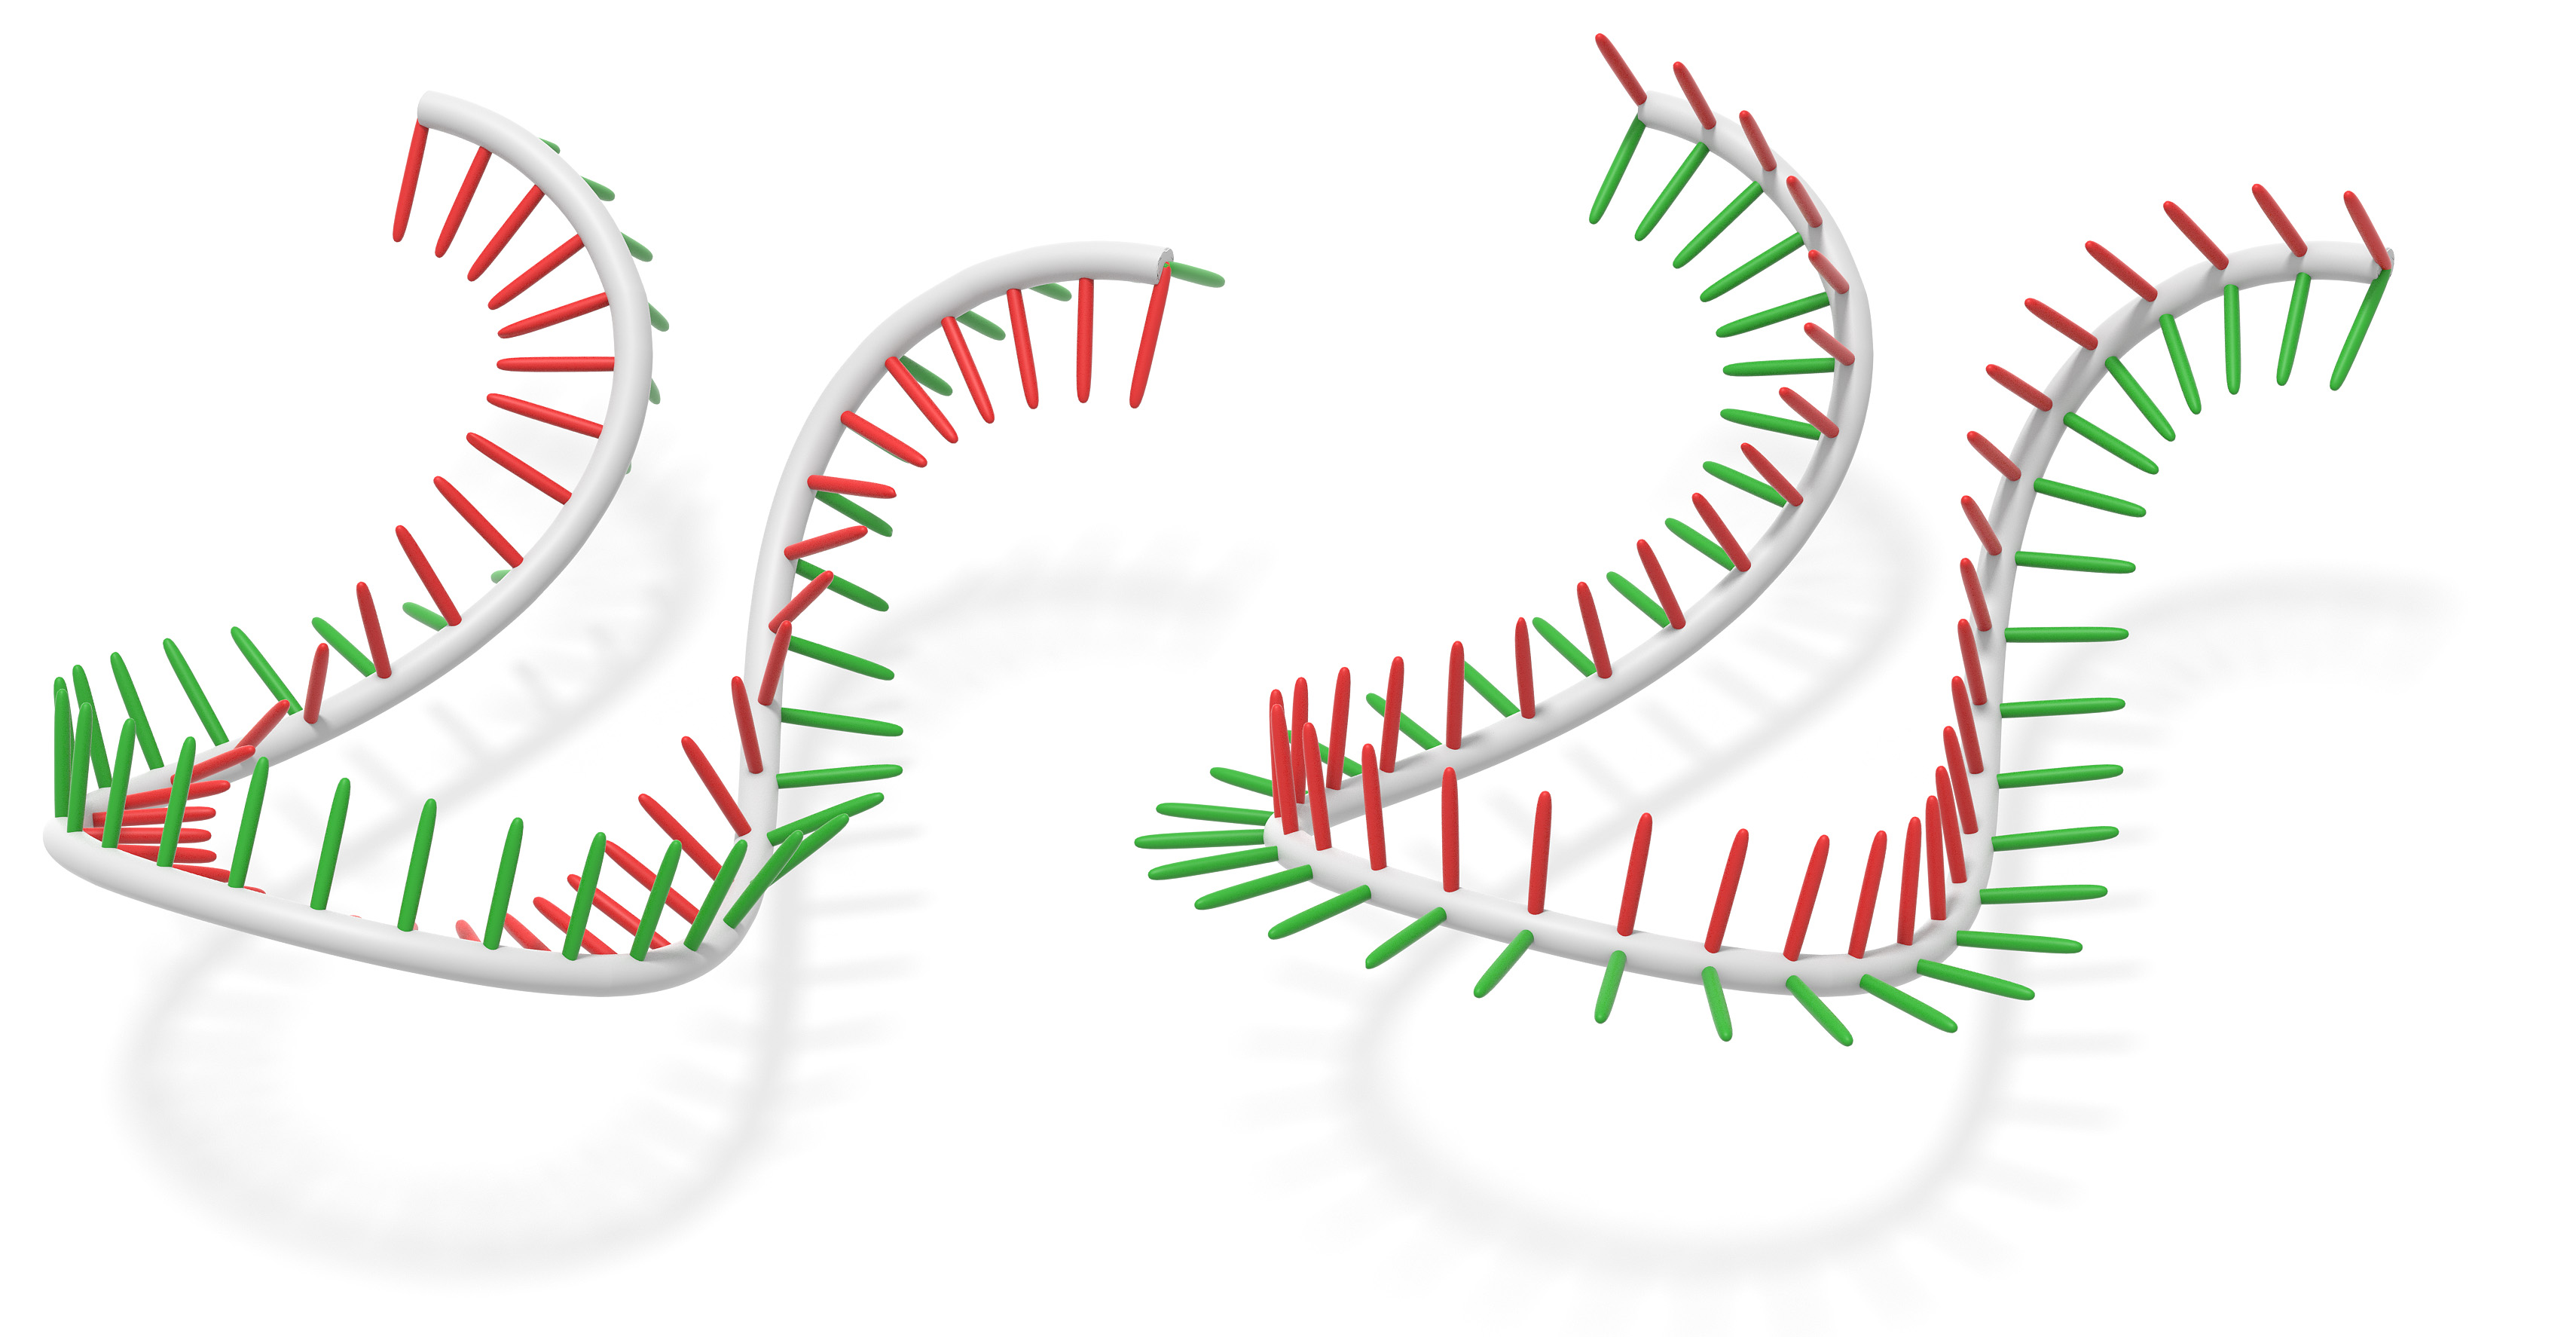
\includegraphics[width=4in]{images/frenet-frame.jpg}
   \caption{If we use the Frenet frame \emph{(left)} to twist fibers around the yarn, the twists will be uneven, since the frame itself exhibits significant nonuniform twist.  Adjusting the Frenet frame \emph{(right)} gives us a more parallel frame, which in turn enables us to define uniformly-twisted fibers.}
   \label{fig:frenet-frame}
\end{figure}

The resulting fiber curve now twists uniformly along the entire loop:
\begin{center}
   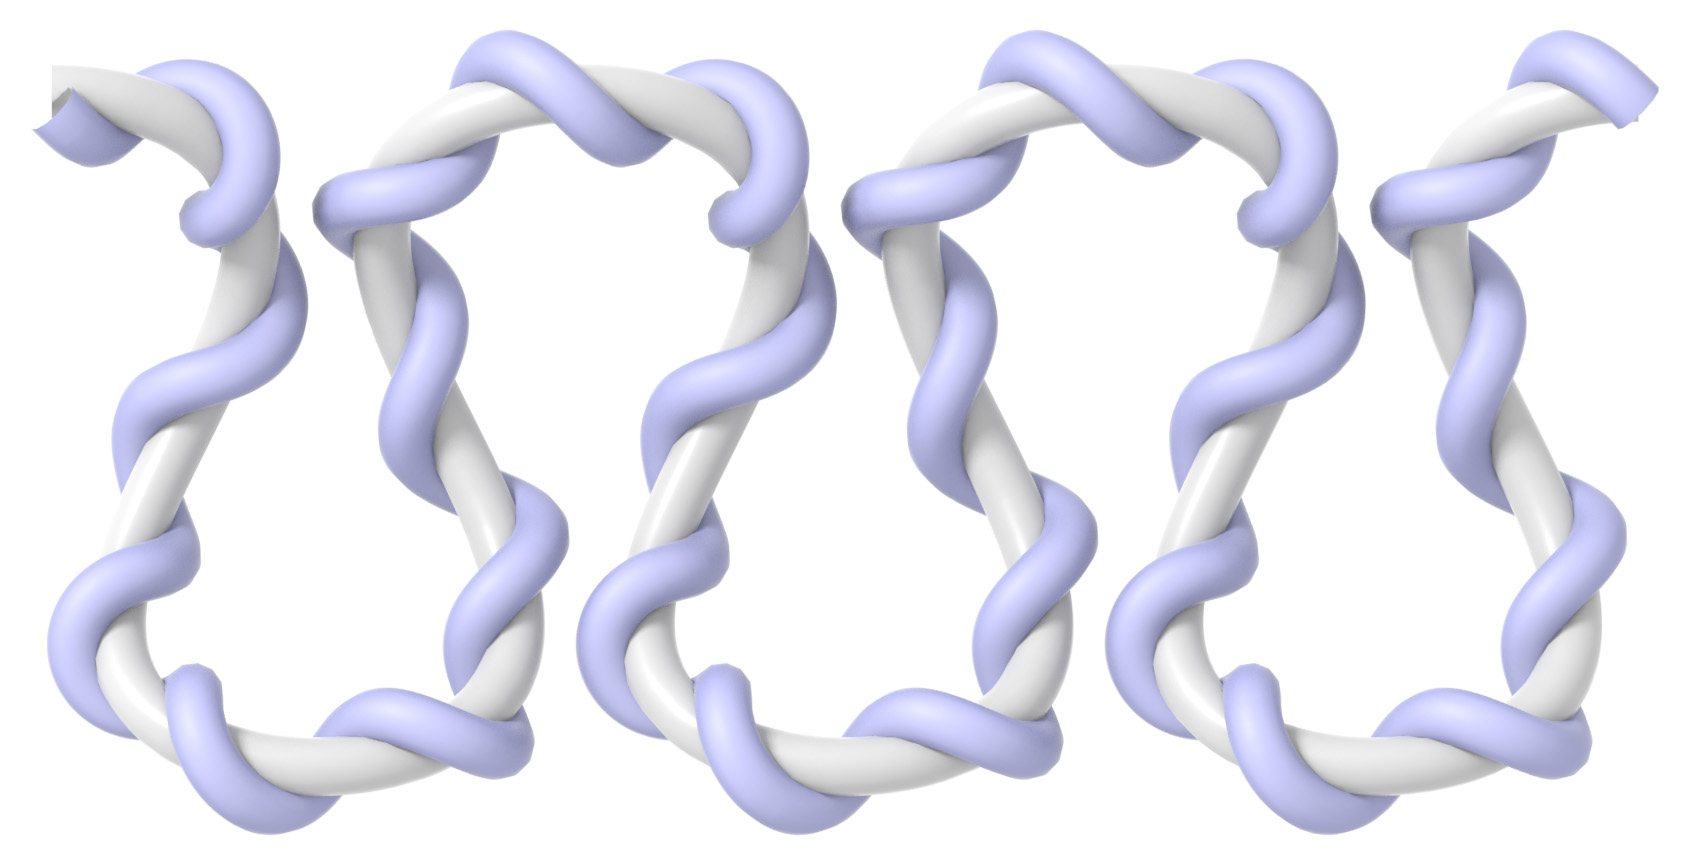
\includegraphics[width=2.5in]{images/fiber-even.jpg}
\end{center}
Finally, to fill in the rest of the yarn, we can draw several copies of the fiber curve where the phase has been shifted by uniform increments \(\phi\).  Our final fiber curve is then given by
\begin{equation}
   \label{eq:FiberCurve}
   \boxed{\eta_\phi(t) := \gamma(t) + r( \cos(\theta_\phi(t)) e_2(t) + \sin(\theta_\phi(t)) e_3(t) ),}
\end{equation}
where
\[ 
      \theta_\phi(t) := \omega t - 2\cos(t) + \phi.
\]
Figure~\ref{fig:fibers-example} shows an example.

\begin{figure}[h!]
   \centering
   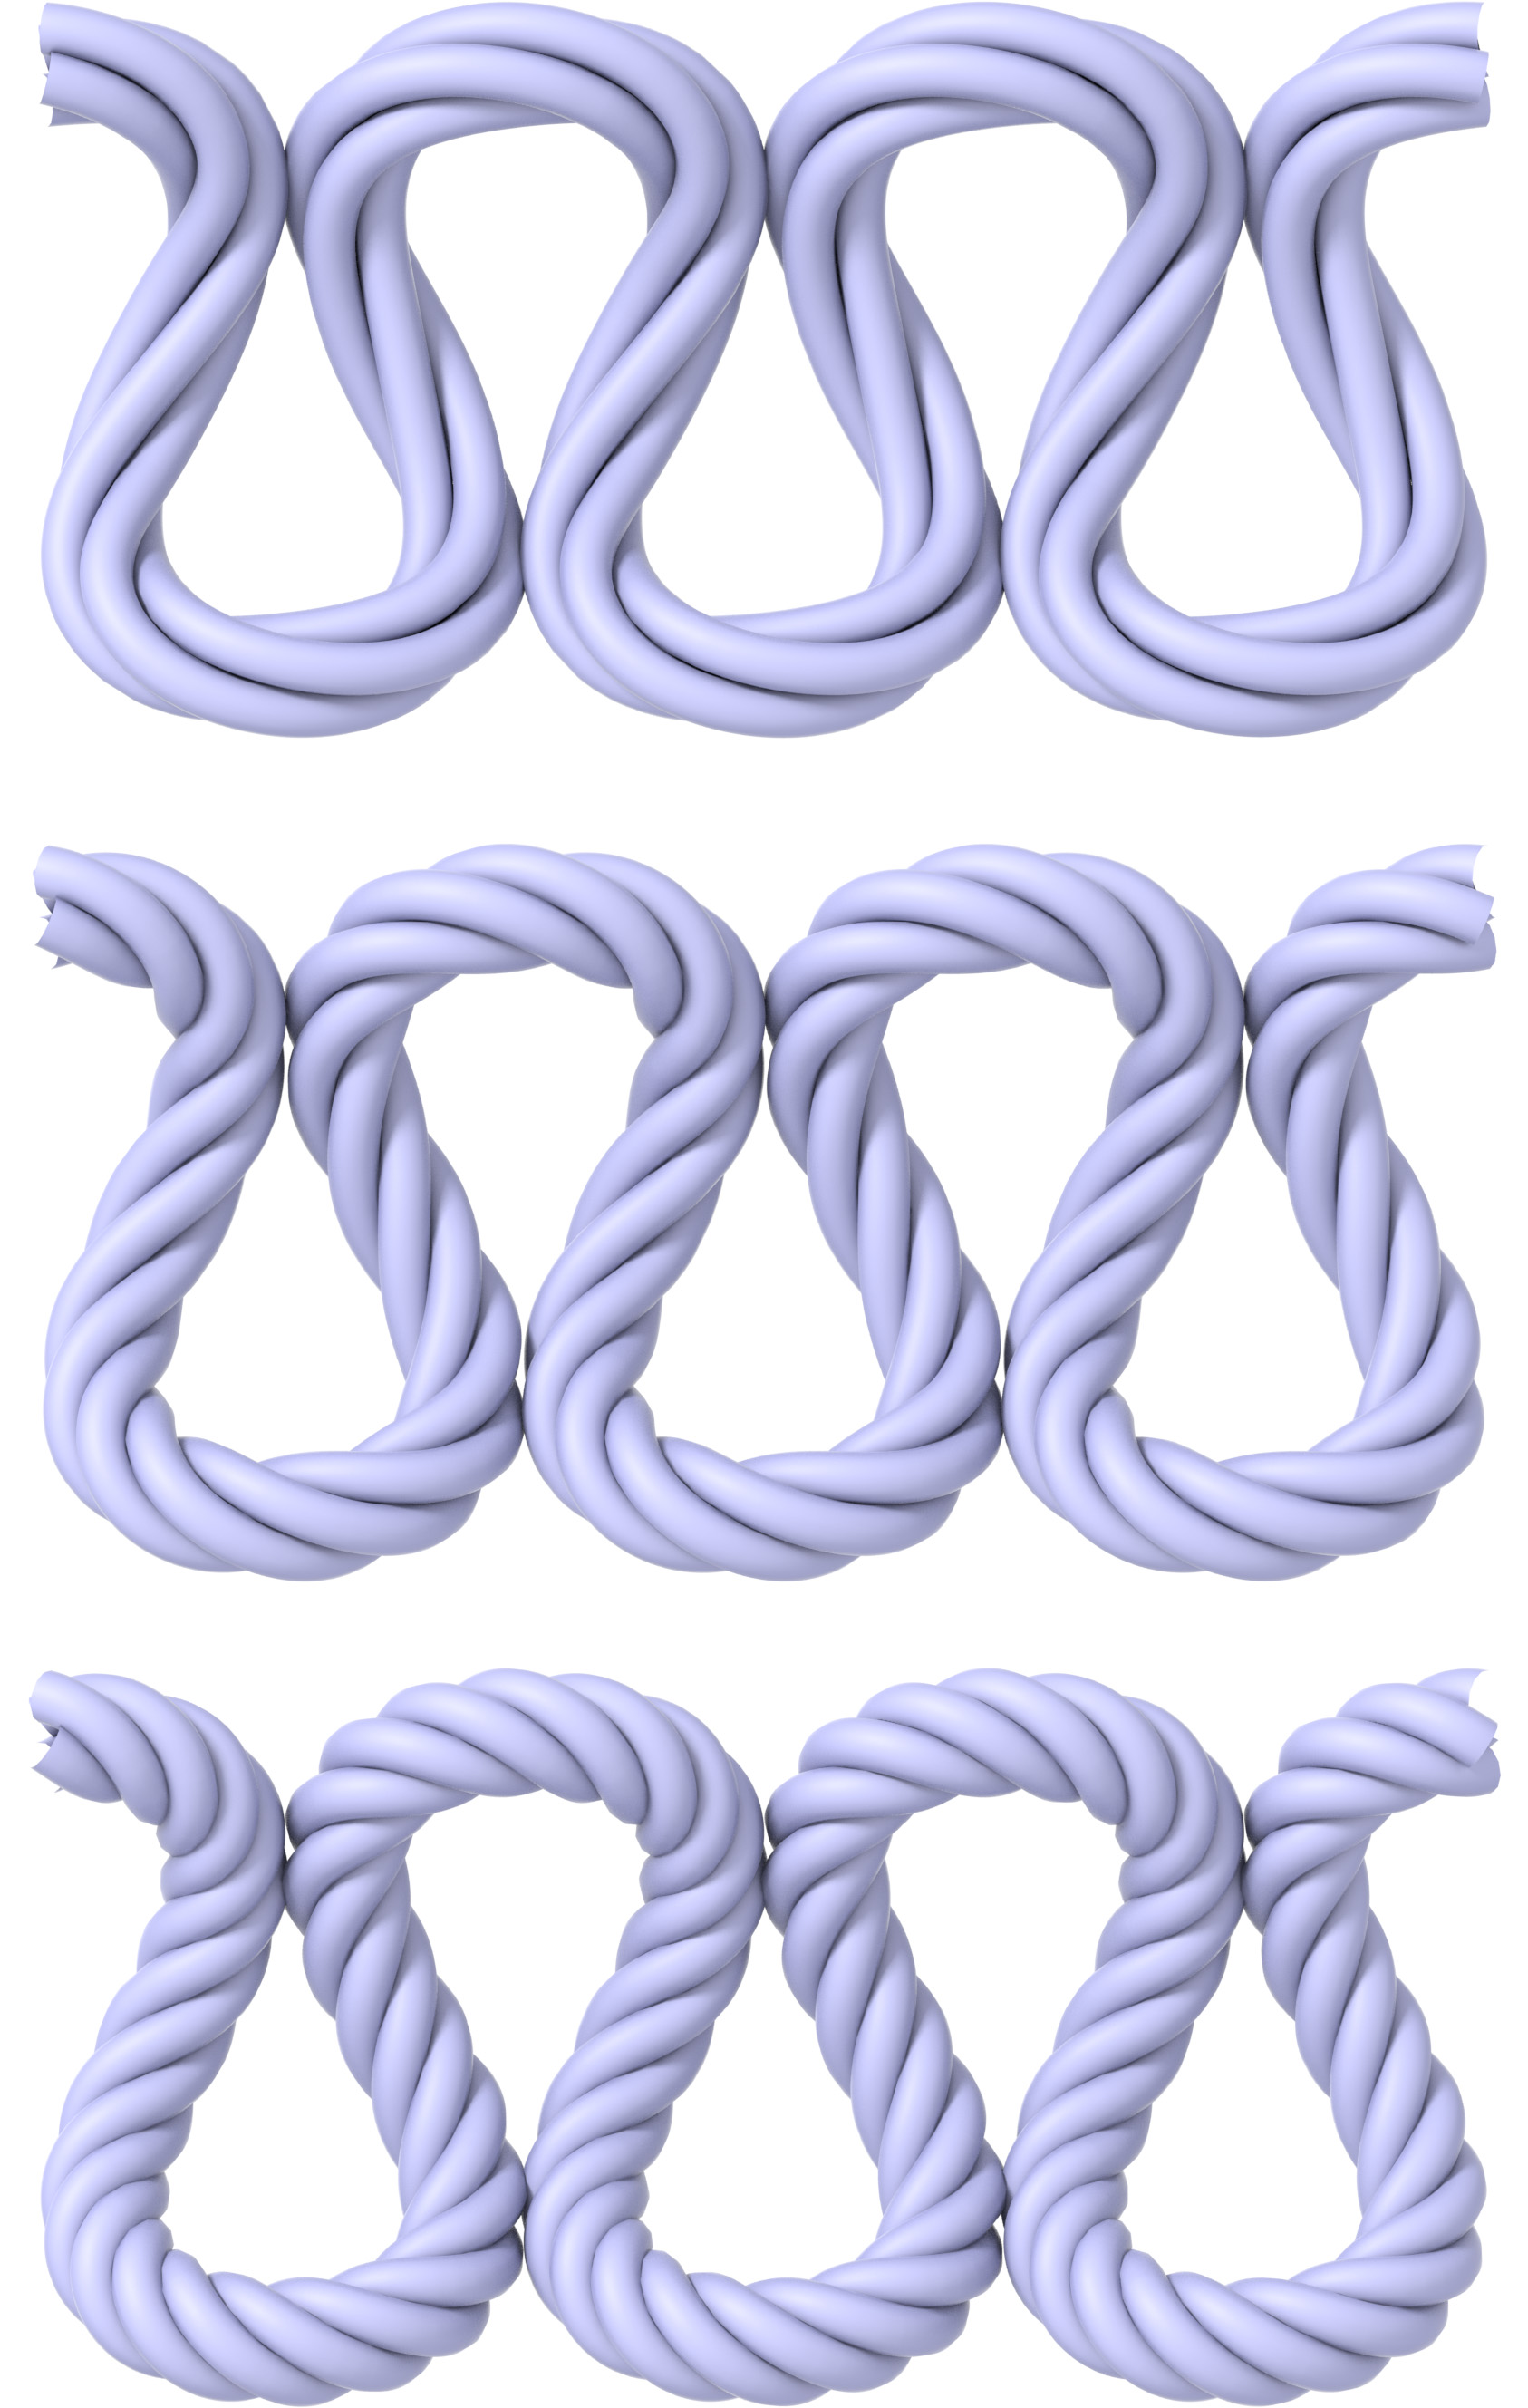
\includegraphics[width=2.5in]{images/fibers-example.jpg}
   \caption{Fiber curves for twist frequencies \(\omega = 2\) \emph{(top)}, \(\omega = 4\) \emph{(middle)}, and \(\omega = 6\) \emph{(bottom)}.  Here \(r = 1/2\) and we plot four fiber curves with phases \(\phi = k\pi/2\), \(k=0,1,2,3\).  The tube radius used for visualization is \(R = 7/20\).\label{fig:fibers-example}}
\end{figure}

\section{Arc Length and Thickness}
\label{sec:ArcLengthAndThickness}

Curve length is useful for anticipating how much yarn will be needed to knit a garment.  Note, however, that since our model is not based on physical equations---and because material properties can vary significantly among yarn types and manufacturing processes---the lengths described here will provide only a rough proxy for the actual quantity of yarn used to knit a real garment.

The arc length \(ds_\gamma\) of the yarn curve \(\gamma(t)\) is given by
\begin{equation}
   \label{eq:YarnArcLength}
   ds_\gamma = \sqrt{(1 + 2a\cos(2 t))^2 + h^2\sin(t)^2 + 4 d^2\sin(2t)^2} dt.
\end{equation}
As with most curves, \(\gamma(t)\) does not admit a closed-form arc-length reparameterization---nor its its arc length even directly integrable.  In contrast to \cite{Peirce:1947:GPA} and \cite{Leaf:1955:GPK}, who give approximations of curve length for their parameterized models, we advocate the use of numerical integration to obtain an accurate estimate of length.  For instance, one could integrate Equation~\ref{eq:YarnArcLength} over the interval \(t \in [0,2\pi]\) using any standard numerical quadrature scheme (e.g., midpoint quadrature) to get the length of a single loop.  Alternatively, the length of a polyline approximation of \(\gamma(t)\) gives a perfectly good (secant) approximation, especially for a large number of sample points.

The tube thickness \(R\) used to give thickness to centerline curves will depend on the curve parameters \(a,h,d,r,\omega\), as well as any physical or aesthetic considerations.  One possible choice is to use the smallest \(R\) such that sweeping a disk of radius \(R\) along the curve (and contained in the plane orthogonal to the curve tangent) will not yield any self-intersections~\cite[Section 3]{gonzalez1999global}.  Like curve length, there is no simple expression for this radius as a function of the curve parameters---if an exact value is needed, one can apply the \emph{octrope} algorithm of \citet{ashton2005fast} to the polygonal approximation provided by the code in Appendix~\ref{app:Code}.

\mbox{}

\paragraph{Acknowledgements.} Thanks to Mark Gillespie and Jim McCann for insightful discussions and useful pointers to early literature on yarn geometry, and to Rob Piek\'{e} for pointing out errors in the original draft.

\bibliographystyle{apalike}
\bibliography{YarnCurve}

\clearpage

\appendix

\section{Displacement Maps}
\label{app:DisplacementMaps}

\begin{figure}[h!]
   \centering
   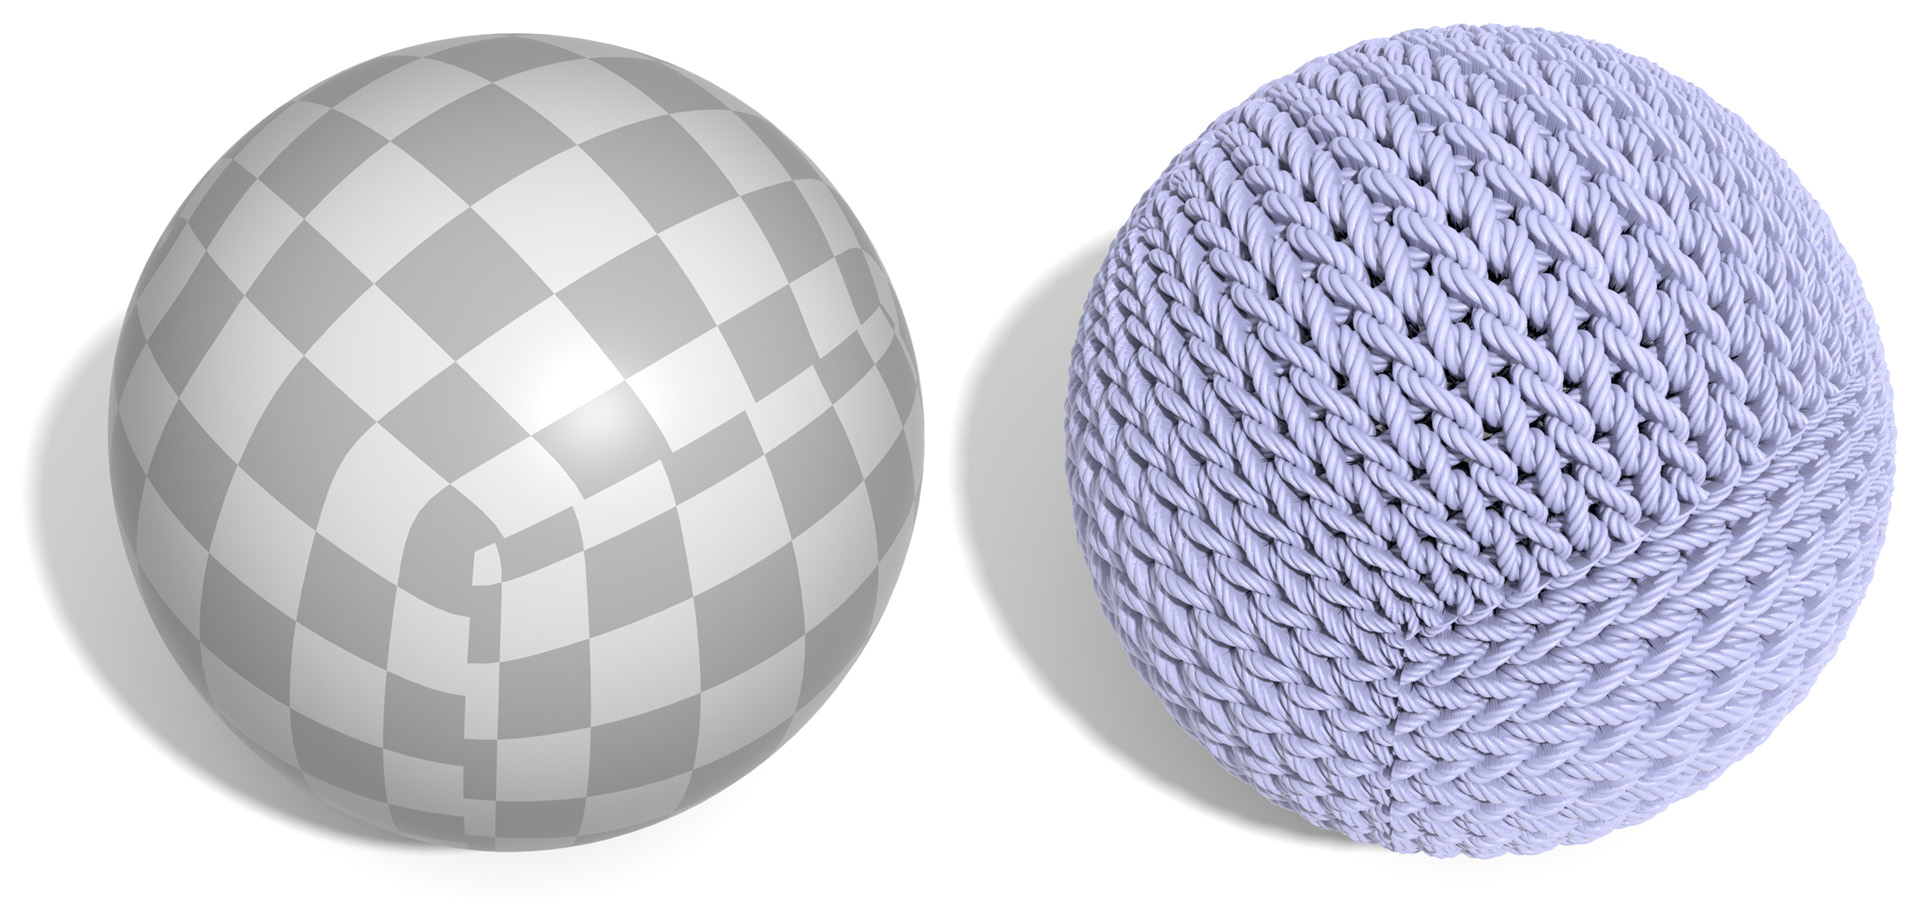
\includegraphics[width=3in]{images/yarn-displacement-example.jpg}
   \caption{Parameterized surface mesh \emph{(left)} rendered with displacement maps based on the yarn fiber geometry \emph{(right)}.\label{fig:yarn-displacement-example}}
\end{figure}

For rendering knit materials, it can be more efficient (or simply convenient) to use a displacement map rather than explicit geometry.  The images below provide tileable patterns for front and back displacements, as well as the associated alpha matte.  An example is shown in Figure~\ref{fig:yarn-displacement-example}.

\begin{center}
   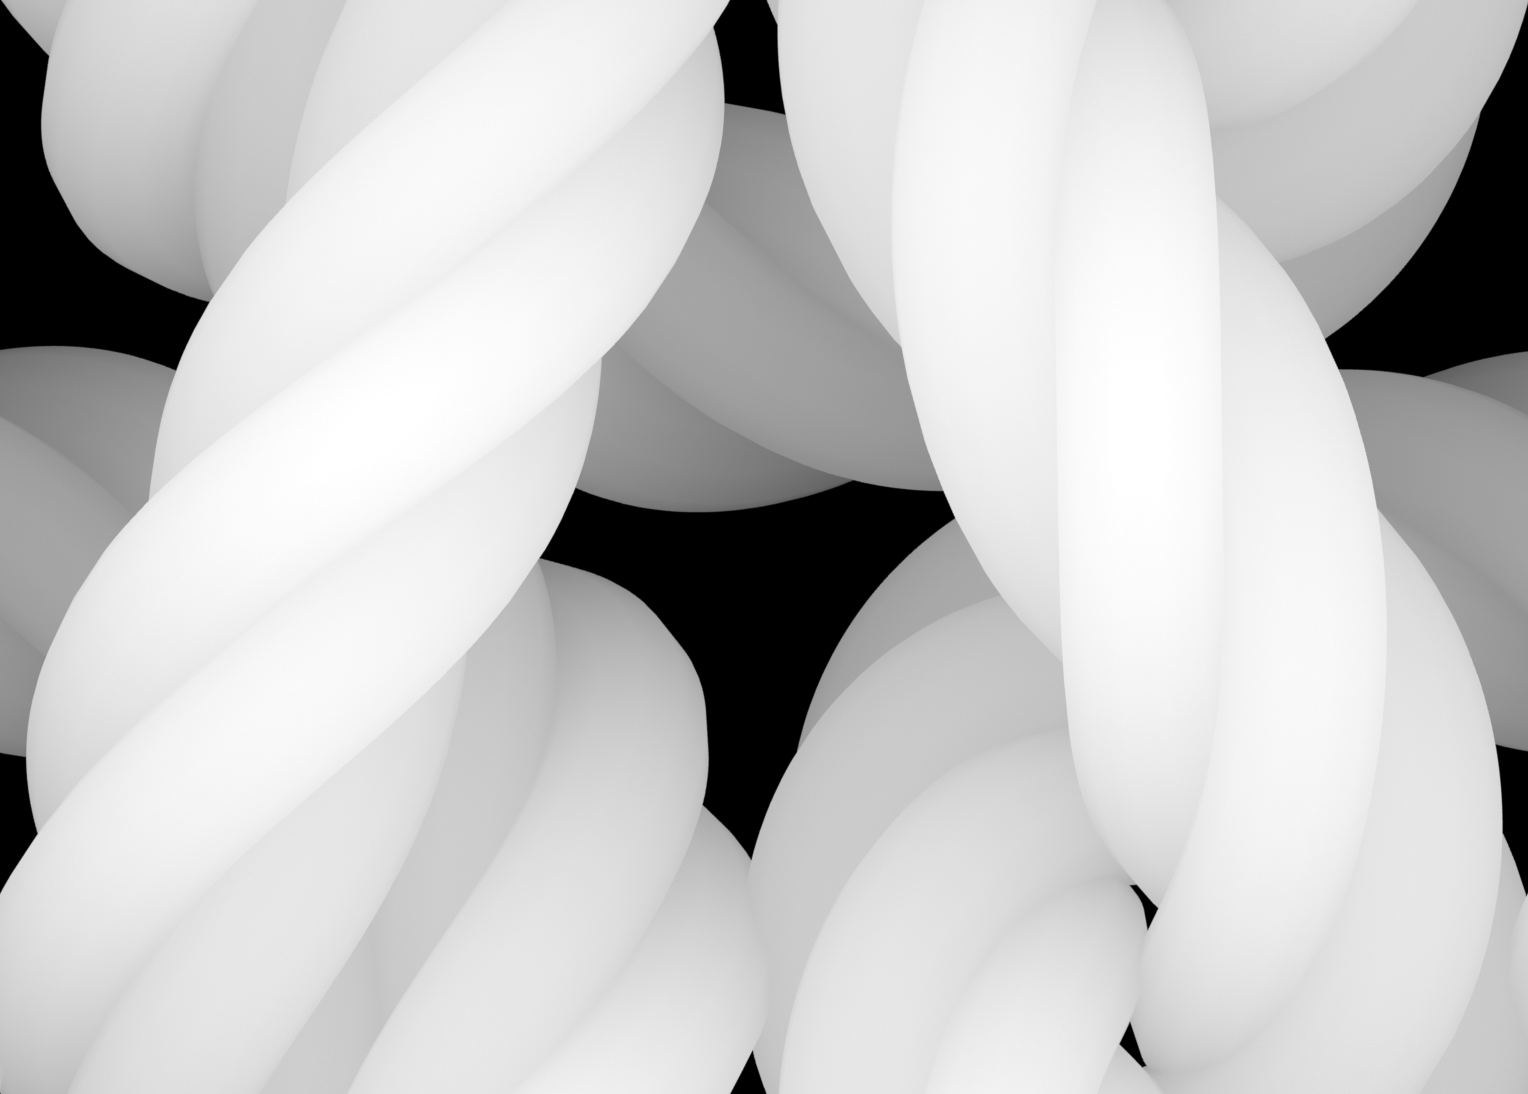
\includegraphics[width=2.75in]{images/yarn-displacement-front.png}

   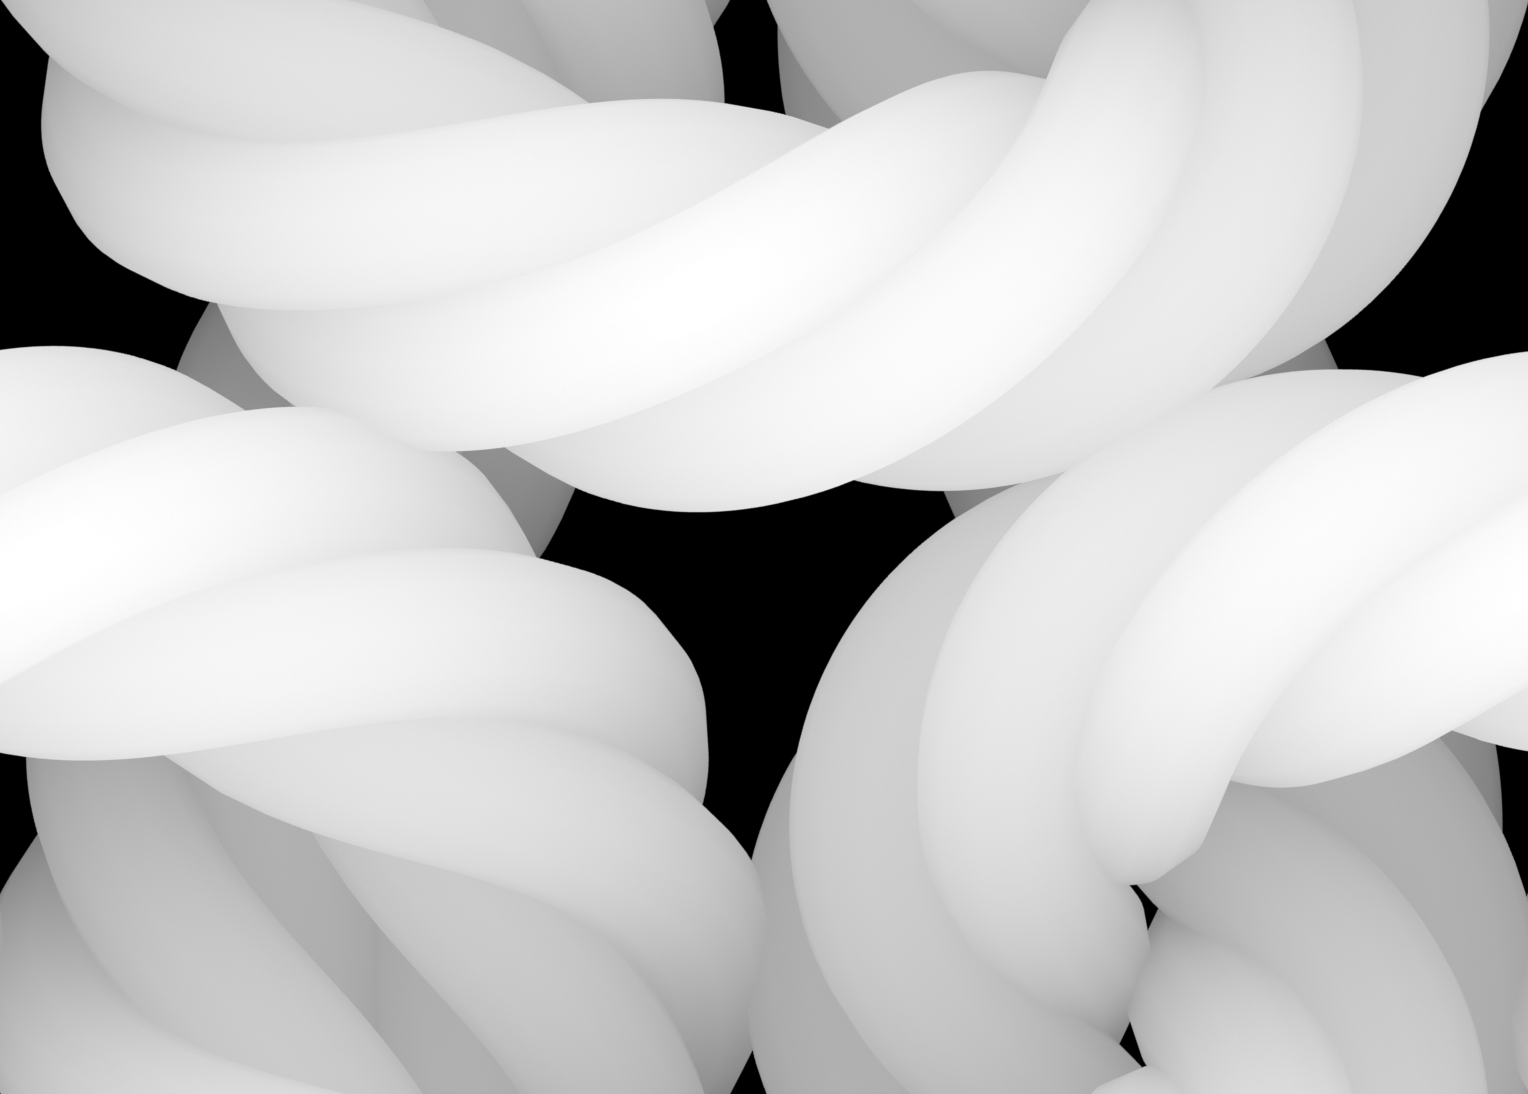
\includegraphics[width=2.75in]{images/yarn-displacement-back.png}

   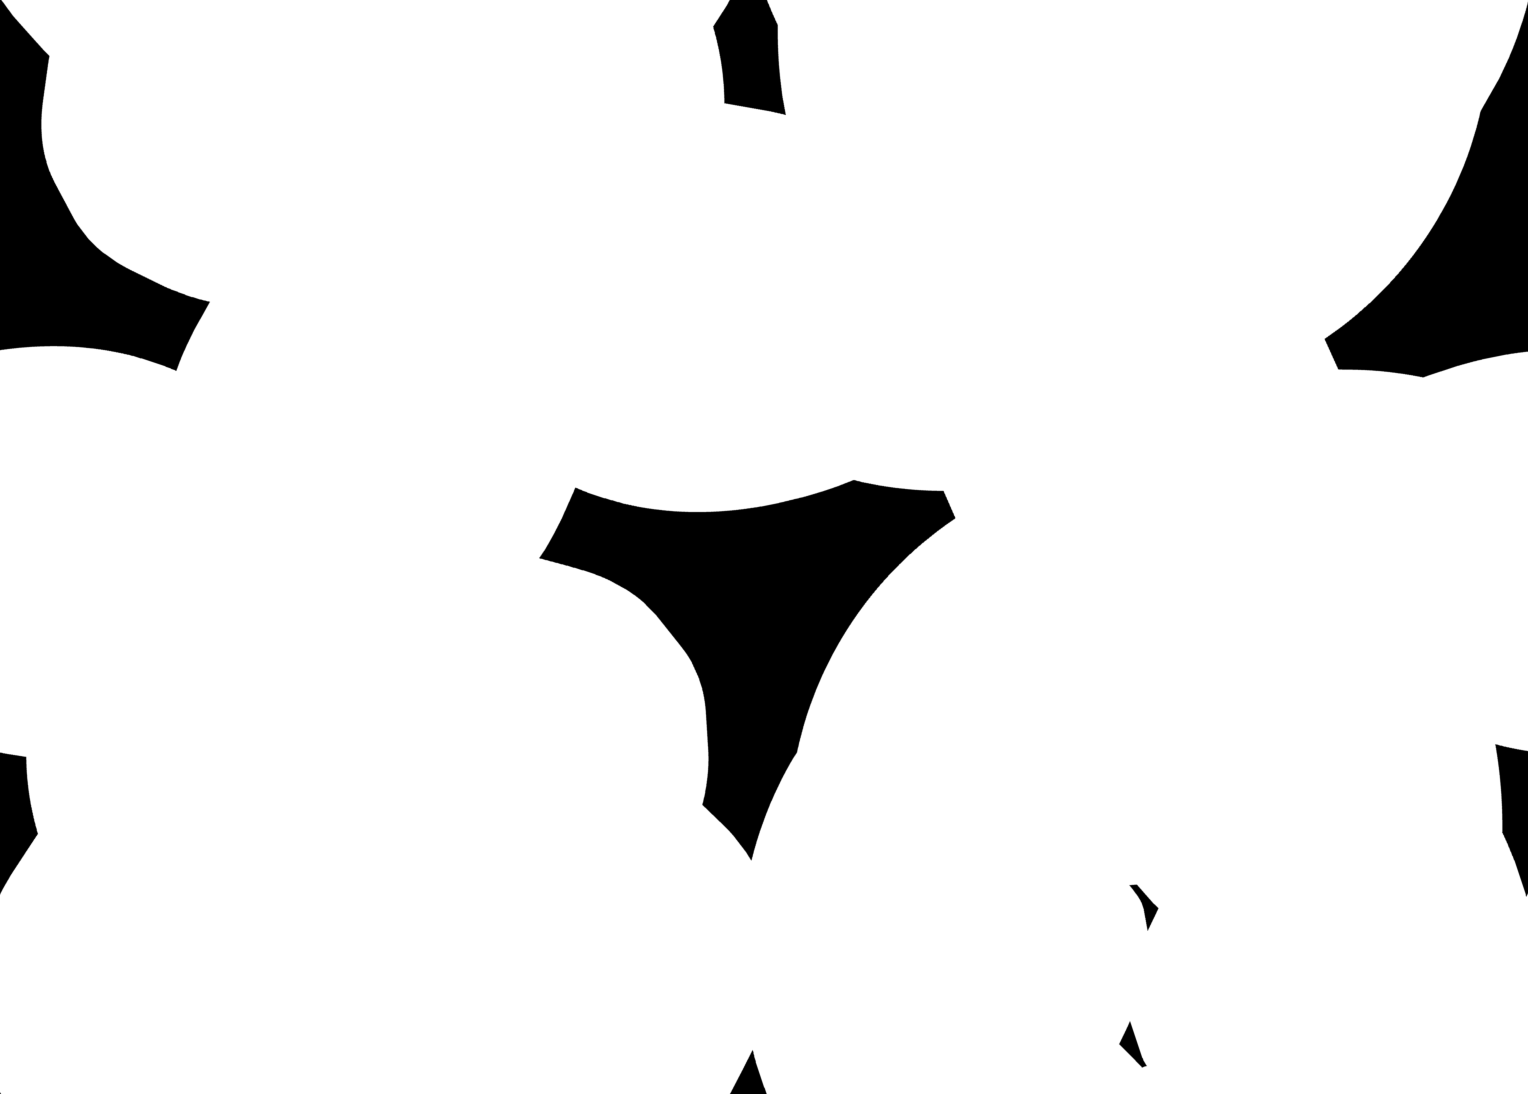
\includegraphics[width=2.75in]{images/yarn-alpha.png}
\end{center}


\clearpage
\pagestyle{empty}

\section{Code}

\definecolor{bg}{rgb}{0.95,0.95,0.95}
\label{app:Code}

\inputminted[bgcolor=bg]{c}{../code/plain-knit.c}

\clearpage

\end{document}
